\documentclass[a4paper]{article}

\input{style/ch_xelatex.tex}
\input{style/scala.tex}

%代码段设置
\lstset{numbers=left,
basicstyle=\tiny,
numberstyle=\tiny,
keywordstyle=\color{blue!70},
commentstyle=\color{red!50!green!50!blue!50},
frame=single, rulesepcolor=\color{red!20!green!20!blue!20},
escapeinside=``
}

\usepackage{ctex}
\usepackage{graphicx}
\usepackage{color,framed}
\usepackage{listings}
\usepackage{caption}
\usepackage{amssymb}
\usepackage{enumerate}
\usepackage{xcolor}
\usepackage{bm}
\usepackage{lastpage}
\usepackage{fancyhdr}
\usepackage{tabularx}
\usepackage{geometry}
\usepackage{graphics}
\usepackage{hyperref}
\usepackage{subfigure}
\usepackage{float}
\usepackage{pdfpages}
\usepackage{pgfplots}
\pgfplotsset{width=10cm,compat=1.9}
\usepackage{multirow}
\usepackage{footnote}
\usepackage{booktabs}

%-----------------------伪代码------------------
\usepackage{algorithm}
\usepackage{algorithmicx}
\usepackage{algpseudocode}
\floatname{algorithm}{Algorithm}
\renewcommand{\algorithmicrequire}{\textbf{Input:}}
\renewcommand{\algorithmicensure}{\textbf{Output:}}
\usepackage{lipsum}
\makeatletter
\newenvironment{breakablealgorithm}
  {% \begin{breakablealgorithm}
  \begin{center}
     \refstepcounter{algorithm}% New algorithm
     \hrule height.8pt depth0pt \kern2pt% \@fs@pre for \@fs@ruled
     \renewcommand{\caption}[2][\relax]{% Make a new \caption
      {\raggedright\textbf{\ALG@name~\thealgorithm} ##2\par}%
      \ifx\relax##1\relax % #1 is \relax
         \addcontentsline{loa}{algorithm}{\protect\numberline{\thealgorithm}##2}%
      \else % #1 is not \relax
         \addcontentsline{loa}{algorithm}{\protect\numberline{\thealgorithm}##1}%
      \fi
      \kern2pt\hrule\kern2pt
     }
  }{% \end{breakablealgorithm}
     \kern2pt\hrule\relax% \@fs@post for \@fs@ruled
  \end{center}
  }
\makeatother
%------------------------代码-------------------
\usepackage{xcolor}
\usepackage{listings}
\lstset{
breaklines,
basicstyle=\small\ttfamily,
keywordstyle=\color{blue!70}\bfseries,
commentstyle=\color{red!50!green!50!blue!50},
stringstyle=\color{orange!80!black},
numbers=left,
numberstyle=\tiny\color{blue!50},
frame=trbl,
rulesepcolor=\color{red!20!green!20!blue!20},
language=Python
}

%-------------------------页面边距--------------
\geometry{a4paper,left=2.3cm,right=2.3cm,top=2.7cm,bottom=2.7cm}
%-------------------------页眉页脚--------------
\usepackage{fancyhdr}
\pagestyle{fancy}
\lhead{\kaishu \leftmark}
% \chead{}
\rhead{\kaishu 机器学习实验报告}%加粗\bfseries
\lfoot{}
\cfoot{\thepage}
\rfoot{}
\renewcommand{\headrulewidth}{0.1pt}
\renewcommand{\footrulewidth}{0pt}%去掉横线
\newcommand{\HRule}{\rule{\linewidth}{0.5mm}}%标题横线
\newcommand{\HRulegrossa}{\rule{\linewidth}{1.2mm}}
\setlength{\textfloatsep}{10mm}%设置图片的前后间距
%--------------------文档内容--------------------

\begin{document}
\renewcommand{\contentsname}{目\ 录}
\renewcommand{\appendixname}{附录}
\renewcommand{\appendixpagename}{附录}
\renewcommand{\refname}{参考文献}
\renewcommand{\figurename}{图}
\renewcommand{\tablename}{表}
\renewcommand{\today}{\number\year 年 \number\month 月 \number\day 日}

%-------------------------封面----------------
\begin{titlepage}
    \begin{center}
    
\includegraphics[width=0.8\textwidth]{NKU.png}\\[1cm]
    \vspace{20mm}
		\textbf{\huge\textbf{\kaishu{计算机学院}}}\\[0.5cm]
		\textbf{\huge{\kaishu{机器学习实验报告}}}\\[2.3cm]
		\textbf{\Huge\textbf{\kaishu{实验七}}}

		\vspace{\fill}

    \centering
    \textsc{\LARGE \kaishu{姓名\ :\ 周重天}}\\[0.5cm]
    \textsc{\LARGE \kaishu{学号\ :\ 2311082}}\\[0.5cm]
    \textsc{\LARGE \kaishu{专业\ :\ 计算机科学与技术}}\\[0.5cm]

    \vfill
    {\Large \today}
    \end{center}
\end{titlepage}

\renewcommand {\thefigure}{\thesection{}.{\arabic{figure}}}%图片按章标号
\renewcommand{\figurename}{图}
\renewcommand{\contentsname}{目录}
\cfoot{\thepage\ of \pageref{LastPage}}%当前页 of 总页数

% 生成目录
\clearpage
\tableofcontents
\newpage


\section{实验目标}

本实验的目标是实现 SegNet 的简化版本，并在多数字 MNIST 数据集上训练和验证该模型。SegNet 是一种经典的深度卷积编码器-解码器网络架构，用于执行像素级别的图像语义分割任务。通过实现这个简化版本的 SegNet，学生需要：深入理解编码-解码网络的设计原理，掌握池化索引在上采样中的应用，实现完整的前向传播和训练流程，并在实际数据集上验证模型的分割性能。

\section{SegNet 简化版的基本原理}

\subsection{整体架构设计}

SegNet 采用对称的编码-解码架构，其核心思想是通过编码器逐步压缩图像到低分辨率的特征表示，随后通过对称的解码器恢复空间细节。与标准的上采样方法（如双线性插值）不同，SegNet 利用编码阶段记录的最大池化索引，在解码阶段进行稀疏上采样，这样可以更有效地保留边界信息和细节特征。

\subsection{编码器（下采样）路径}

编码器由 4 层卷积块组成，每层的结构为：卷积层 $\to$ 批归一化 $\to$ ReLU 激活 $\to$ 最大池化。这个设计的特点是，最大池化使用 \texttt{return\_indices=True} 参数记录每个位置的最大值索引。通过这 4 层递进式的下采样，输入尺寸从 $3 \times 64 \times 64$ 逐步压缩至 $256 \times 4 \times 4$，使特征图不断降采样的同时，通道数逐层增加（32 $\to$ 64 $\to$ 128 $\to$ 256）。

\subsection{解码器（上采样）路径}

解码器同样由 4 层反卷积块组成，结构为：最大反池化 $\to$ 卷积层 $\to$ 批归一化 $\to$ ReLU 激活。解码器的关键特征是它利用编码阶段保存的池化索引，通过 \texttt{MaxUnpool2d} 操作恢复特征图的空间分辨率。这种索引驱动的上采样比简单的双线性插值更能保留物体的清晰边界和细节信息。解码过程将特征图从 $256 \times 4 \times 4$ 逐步恢复至 $32 \times 64 \times 64$，通道数递减（128 $\to$ 64 $\to$ 32 $\to$ 32）。

\subsection{最终分类层}

在解码器的最后，使用一个 $1 \times 1$ 卷积层将 32 通道的特征映射到 11 个类别（背景 + 10 个数字）的分割结果。这个卷积层带有偏差项，允许模型学习类别之间的判别特征。

\section{实现的训练验证过程}

\subsection{下采样路径的实现}

下采样路径通过循环构造 4 个卷积块，每个块包含卷积层、批归一化和最大池化。实现代码如下：

\begin{lstlisting}
for i in range(self.num_down_layers):
    layers_conv_down.append(
        nn.Conv2d(
            in_channels=input_size,
            out_channels=down_filter_sizes[i],
            kernel_size=kernel_sizes[i],
            padding=conv_paddings[i],
            bias=False,
        )
    )
    layers_bn_down.append(nn.BatchNorm2d(down_filter_sizes[i]))
    layers_pooling.append(
        nn.MaxPool2d(
            kernel_size=pooling_kernel_sizes[i],
            stride=pooling_strides[i],
            return_indices=True,
        )
    )
    input_size = down_filter_sizes[i]
\end{lstlisting}

这段代码实现的是 SegNet 编码器（编码部分）的构建。通过循环遍历参数，逐层构造 4 个卷积块，每个块包含卷积层、批归一化和最大池化三个组件。这 4 层编码器从上往下逐步压缩图像分辨率，将输入从 $3 \times 64 \times 64$ 压缩到 $256 \times 4 \times 4$，同时提取和浓缩图像的高层次语义特征。

以下是 \texttt{return\_indices=True}，这是 SegNet 的核心创新之一。当我们进行最大池化时，通常只输出最大值，但这会丢失位置信息。通过 \texttt{return\_indices=True}，我们记录下每个最大值在原始特征图中的位置。比如说，一个 $2 \times 2$ 的池化操作会将 4 个数中的最大值输出，同时记下这个最大值来自 4 个数中的哪一个。这些位置信息会在后续的解码过程中被重复使用，让网络能够精确地恢复出细节。

卷积层的 \texttt{bias=False} 参数看似简单，却体现了一个重要的网络设计原则。在卷积层之后紧跟着批归一化层（\texttt{BatchNorm2d}），而批归一化层本身就包含了可学习的偏差参数。如果卷积层也加入偏差，就会产生冗余——两层都在学习偏差，这会增加计算量并可能导致训练不稳定。因此，我们在卷积层中禁用偏差，让批归一化层单独负责调整特征的均值和方差。

整个下采样过程采用了循环参数化的设计。注意代码中通过循环遍历 \texttt{down\_filter\_sizes} 和其他参数列表来构建每一层。这意味着如果我们想要改变网络的深度（层数）或通道数配置，只需要修改参数列表，无需改动代码逻辑。这样的设计提高了代码的灵活性和复用性。在这个实现中，输入图像被逐步压缩：从 $3 \times 64 \times 64$ 经过第一层编码器变成 $32 \times 32 \times 32$，再经过第二层变成 $64 \times 16 \times 16$，继续压缩到 $128 \times 8 \times 8$，最后编码成 $256 \times 4 \times 4$ 的紧凑特征表示。

\subsection{上采样路径的实现}

上采样路径对称地构造 4 个反卷积块，每块包含最大反池化、卷积层和批归一化。实现代码如下：

\begin{lstlisting}
for i in range(self.num_up_layers):
    layers_unpooling.append(
        nn.MaxUnpool2d(
            kernel_size=pooling_kernel_sizes[-(i + 1)],
            stride=pooling_strides[-(i + 1)],
        )
    )
    layers_conv_up.append(
        nn.Conv2d(
            in_channels=input_size,
            out_channels=up_filter_sizes[i],
            kernel_size=kernel_sizes[-(i + 1)],
            padding=conv_paddings[-(i + 1)],
            bias=False,
        )
    )
    layers_bn_up.append(nn.BatchNorm2d(up_filter_sizes[i]))
    input_size = up_filter_sizes[i]
\end{lstlisting}

这段代码实现了解码器的对称结构，同样有三个关键设计点。

第一，最大反池化层（\texttt{MaxUnpool2d}）的作用是"反向"编码器中的最大池化。它不是用简单的插值方法（如双线性插值）来扩大特征图，而是使用编码阶段保存的那些池化索引。具体来说，它知道编码时每个最大值来自哪个位置，现在就把这个最大值放回那个位置，其他地方填零。这样可以非常精确地恢复特征图的空间结构，特别是对于物体的边界信息保留得很好。

第二，代码中大量使用了反向索引 \texttt{-(i + 1)}。这是一个巧妙的设计：编码器按顺序使用参数列表的前 4 个元素，解码器则按相反的顺序使用，从最后一个元素开始向前。例如，编码器用 \texttt{pooling\_kernel\_sizes[0]} 作为第一层的池化核大小，而解码器用 \texttt{pooling\_kernel\_sizes[-1]}（最后一个元素）作为最后一层反池化的核大小。这确保了编码和解码是完全对称的：如果编码中某一层把图像缩小了 2 倍，解码中对应的层就会把它放大 2 倍。这种对称性是 SegNet 设计的精妙之处。

第三，卷积层的其他参数（卷积核大小 \texttt{kernel\_sizes}、填充 \texttt{conv\_paddings} 等）也都采用同样的反向索引策略。这保证了解码路径中的卷积层与编码路径完全对应。通过这种精心的对称设计，特征可以被完整而准确地编码成低分辨率的紧凑表示，然后再完整而准确地解码回原始分辨率，中间不会丢失关键的空间细节信息。

\subsection{前向传播函数的实现}

前向传播函数实现了完整的编码-解码过程，关键是正确管理和利用池化索引：

\begin{lstlisting}
def forward(self, x):
    pooling_indices = []
    pooling_sizes = []
    
    for i in range(self.num_down_layers):
        x = self.layers_conv_down[i](x)
        x = self.layers_bn_down[i](x)
        x = self.relu(x)
        pooling_sizes.append(x.size())
        x, indices = self.layers_pooling[i](x)
        pooling_indices.append(indices)
    
    for i in range(self.num_up_layers):
        j = self.num_up_layers - 1 - i
        x = self.layers_unpooling[i](x, pooling_indices[j], 
            output_size=pooling_sizes[j])
        x = self.layers_conv_up[i](x)
        x = self.layers_bn_up[i](x)
        x = self.relu(x)
    
    x = self.conv_final(x)
    return x
\end{lstlisting}

前向传播函数是整个网络的核心控制逻辑，它需要协调编码和解码的过程，并确保池化索引被正确地传递和使用。

在编码阶段，函数逐层通过卷积、批归一化和激活，然后执行最大池化。每次池化前，我们记录下当前特征图的大小（用 \texttt{pooling\_sizes.append(x.size())} 保存）。然后执行最大池化，获得两个输出：池化后的特征 \texttt{x} 和池化索引 \texttt{indices}。这个索引就像一份"地图"，记录了哪些位置包含最大值。我们把这份地图存储在 \texttt{pooling\_indices} 列表中以备后用。

在解码阶段，我们需要反向操作。关键的一点是配对关系：解码器的第 $i$ 层应该使用编码器第 $j$ 层保存的索引，其中 $j = \text{num\_up\_layers} - 1 - i$。这确保了完全的对称性。例如，如果解码器的第 0 层（最底部）应该使用编码器的第 3 层（最底部）的索引，这个计算公式就会正确地给出这个配对。

最大反池化 \texttt{MaxUnpool2d} 函数接收三个参数：待解码的特征 \texttt{x}、对应的池化索引 \texttt{pooling\_indices[j]}，以及目标输出尺寸 \texttt{output\_size=pooling\_sizes[j]}。它会根据这些信息，把压缩的特征精确地还原回编码时的大小。之后，我们再依次通过卷积、批归一化和激活函数，就完成了一层解码。

最终，通过一个 $1 \times 1$ 卷积（\texttt{conv\_final}）将最后的 32 通道特征映射到 11 个类别的分割结果。

\subsection{最终卷积层的实现}

最终卷积层用于生成分割逻辑（logits）：

\begin{lstlisting}
self.conv_final = nn.Conv2d(input_size, 11, kernel_size=1, 
    padding=0, bias=True)
\end{lstlisting}

这是一个标准的 $1 \times 1$ 卷积，将最后一层解码器的 32 通道特征映射到 11 个分类通道（背景加 10 个数字类）。与下采样和上采样层不同，这里 \texttt{bias=True}，允许模型学习每个类别的分类偏差。

\subsection{训练过程}


\subsubsection{训练配置和优化策略}

模型在 CPU 上进行训练，使用交叉熵损失函数（CrossEntropy2D）作为优化目标。训练脚本 \texttt{train\_mnist.py} 设置了种子值（seed=37）以确保可复现性。每个 epoch 包含 200 个批次，训练数据通过多个 worker（num\_workers=4）并行加载。优化器使用 PyTorch 标准设置，学习率通过训练脚本的默认配置确定。模型采用定期验证策略，每个 epoch 后都会在验证集上评估性能并保存最优模型。

\subsubsection{训练过程的观察}

下面展示了训练过程中多个 epoch 的典型输出，从初期学习到后期收敛的完整演变：

\begin{lstlisting}[language=bash]
# Epoch 0 - 初期学习阶段
Epoch: [0][0/200]   Time 3.748s (3.748s)   Speed 8.5 samples/s    Loss 2.86586 (2.86586)
Epoch: [0][50/200]  Time 0.338s (0.405s)   Speed 94.8 samples/s   Loss 1.40468 (1.96626)
Epoch: [0][100/200] Time 0.339s (0.366s)   Speed 94.5 samples/s   Loss 0.76594 (1.51711)
Epoch: [0][150/200] Time 0.333s (0.355s)   Speed 96.2 samples/s   Loss 0.44852 (1.21153)
Epoch: [0][190/200] Time 0.321s (0.349s)   Speed 99.6 samples/s   Loss 0.30659 (1.03556)
Mean IoU score: 0.163

# Epoch 1 - 中期学习阶段
Epoch: [1][0/200]   Time 3.563s (3.563s)   Speed 9.0 samples/s    Loss 0.28063 (0.28063)
Epoch: [1][50/200]  Time 0.323s (0.388s)   Speed 99.2 samples/s   Loss 0.26304 (0.25605)
Epoch: [1][100/200] Time 0.327s (0.365s)   Speed 98.0 samples/s   Loss 0.15875 (0.23007)
Epoch: [1][150/200] Time 0.326s (0.354s)   Speed 98.1 samples/s   Loss 0.13822 (0.21096)
Epoch: [1][190/200] Time 0.331s (0.349s)   Speed 96.6 samples/s   Loss 0.13880 (0.19896)
Mean IoU score: 0.274

# Epoch 2 - 后期学习阶段
Epoch: [2][0/200]   Time 3.856s (3.856s)   Speed 8.3 samples/s    Loss 0.11504 (0.11504)
Epoch: [2][50/200]  Time 0.325s (0.405s)   Speed 98.6 samples/s   Loss 0.10145 (0.11837)
Epoch: [2][100/200] Time 0.333s (0.370s)   Speed 96.1 samples/s   Loss 0.08274 (0.10790)
Epoch: [2][150/200] Time 0.324s (0.360s)   Speed 98.5 samples/s   Loss 0.07650 (0.10177)
Epoch: [2][190/200] Time 0.323s (0.360s)   Speed 98.9 samples/s   Loss 0.06933 (0.09827)
Mean IoU score: 0.520
\end{lstlisting}

为了更清楚地观察训练过程中的指标变化，下表总结了多个 epoch 的关键性能指标：

\begin{table}[H]
    \centering
    \begin{tabular}{|c|c|c|c|c|}
    \hline
    \textbf{Epoch} & \textbf{初始损失} & \textbf{最终损失} & \textbf{验证 Loss} & \textbf{验证 IoU} \\
    \hline
    0 & 2.866 & 1.036 & 0.532 & 0.163 \\
    \hline
    1 & 0.281 & 0.199 & 0.325 & 0.274 \\
    \hline
    2 & 0.115 & 0.098 & 0.267 & 0.520 \\
    \hline
    3 & 0.055 & 0.042 & 0.127 & 0.708 \\
    \hline
    4 & 0.028 & 0.027 & 0.081 & 0.819 \\
    \hline
    5 & 0.022 & 0.021 & 0.071 & 0.831 \\
    \hline
    6 & 0.027 & 0.016 & 0.066 & 0.841 \\
    \hline
    7 & 0.015 & 0.013 & 0.067 & 0.839 \\
    \hline
    8 & 0.013 & 0.012 & 0.058 & 0.860 \\
    \hline
    9 & 0.011 & 0.010 & 0.056 & 0.864 \\
    \hline
    10 & 0.008 & 0.009 & 0.057 & 0.861 \\
    \hline
    11 & 0.007 & 0.009 & 0.061 & 0.856 \\
    \hline
    12 & 0.007 & 0.008 & 0.061 & 0.858 \\
    \hline
    13 & 0.007 & 0.013 & 0.138 & 0.702 \\
    \hline
    14 & 0.018 & 0.013 & 0.081 & 0.809 \\
    \hline
    15 & 0.011 & 0.011 & 0.060 & 0.858 \\
    \hline
    16 & 0.011 & 0.009 & 0.053 & 0.872 \\
    \hline
    17 & 0.010 & 0.008 & 0.054 & 0.872 \\
    \hline
    18 & 0.006 & 0.007 & 0.055 & 0.873 \\
    \hline
    19 & 0.006 & 0.007 & 0.056 & 0.870 \\
    \hline
    \end{tabular}
    \caption{20 个 epoch 训练过程中的关键性能指标变化。}
    \label{table:training_progress}
\end{table}

\subsubsection{训练趋势分析}

观察 20 个 epoch 的完整训练过程，模型展现出了典型的深度学习收敛特性：

\textbf{第 0 - 2 个 epoch（快速降损阶段）}：模型处于初期学习阶段。损失值从 2.866 快速下降至 0.098，跌幅达 96.6\%。此时验证 IoU 从 0.163 跃升至 0.520，增幅达 219\%。这表明模型在极短的时间内已经学会了数字与背景的基本区分特征。

\textbf{第 3 - 9 个 epoch（稳健改进阶段）}：模型进入中期学习阶段，性能持续稳定提升。验证 IoU 从 0.708 渐进式增长至 0.864，每个 epoch 的改进幅度约为 2-3\%。训练损失保持在 0.008 - 0.055 之间的低位，验证损失稳定在 0.056 - 0.127 的范围。这一阶段的特点是学习速度适中、性能提升稳定、没有过度波动。

\textbf{第 10 - 12 个 epoch（平台期）}：模型性能在 0.856 - 0.864 之间波动，验证 IoU 基本保持稳定。损失值继续维持低位（0.007 - 0.009）。这说明模型已经逐渐趋向收敛，大多数有效的特征已被充分学习。

\textbf{第 13 个 epoch（异常波动）}：这是训练过程中的一个有趣现象。验证 IoU 突然下跌至 0.702，验证损失激增至 0.138（比平常高 2 倍多）。这种现象在深度学习中通常称为"梯度尖刺"（gradient spike），可能由单个困难样本、学习率调整或数据分布的临时偏差引起。尽管如此，训练损失仍保持低位（0.013），说明模型在训练数据上仍有良好表现。

\textbf{第 14 - 19 个 epoch（恢复与稳定）}：经过第 13 个 epoch 的波动后，模型快速恢复并继续改进。验证 IoU 从 0.809 反弹至 0.873，最终在第 18 个 epoch 达到峰值 0.873（对应验证损失 0.055）。随后的 epoch 19 显示 IoU 略微下降至 0.870，但仍处于历史高位，这表明模型已基本收敛并达到最优性能。
\tab 模型的学习曲线呈"陡峭-平缓-波动-稳定"的典型模式，前 2 个 epoch 实现了性能的快速跃升，随后 7 个 epoch 实现稳健改进，最后 11 个 epoch 中虽有波动但整体趋势向好。训练损失与验证损失的偏差始终保持在合理范围内（最大不超过 0.082），说明模型没有严重过拟合，泛化能力良好。最终的验证 Mean IoU 为 0.873（87.3\%），平均验证损失为 0.056，这代表了该模型在多数字 MNIST 分割任务上的最佳性能。整个训练过程共耗时约 40 分钟，充分验证了 SegNet 池化索引机制在像素级分割中的有效性。


\subsection{验证过程}

\subsubsection{验证配置}

验证脚本 \texttt{validate\_mnist.py} 加载最优模型 \texttt{model\_best.pth.tar}，在完整的验证集（200 个样本）上进行评估。验证过程不进行梯度计算，仅以推理模式运行，使用单个 worker 加载数据。验证集与训练集采用相同的预处理，确保评估的准确性。

\subsubsection{验证性能指标}

验证过程计算两个关键指标：交叉熵损失和 Mean IoU。下面是验证脚本的终端输出的部分信息：

\begin{lstlisting}[language=bash]
=> loading model from out/model_best.pth.tar
=> load 200 samples
Test: [0/200]   Time 3.256 (3.256)      Loss 0.0511 (0.0511)
Test: [10/200]  Time 0.011 (0.310)      Loss 0.0065 (0.0455)
Test: [20/200]  Time 0.010 (0.167)      Loss 0.0239 (0.0530)
Test: [30/200]  Time 0.008 (0.117)      Loss 0.0453 (0.0547)
...
Test: [180/200] Time 0.012 (0.029)      Loss 0.0480 (0.0551)
Test: [190/200] Time 0.013 (0.028)      Loss 0.0265 (0.0550)
Mean IoU score: 0.873
\end{lstlisting}

根据最新的验证运行结果，模型在验证集上的平均损失为 0.0550，表明预测的置信度和准确性都很高。此时每个批次的损失值保持在 0.005 到 0.208 之间的较低范围，其中大多数样本的损失远低于平均值，仅有少数样本（如第 110 批次）出现较高的损失值。

\section{模型分割可视化效果图及观察解释}

\begin{figure}[H]
    \centering
    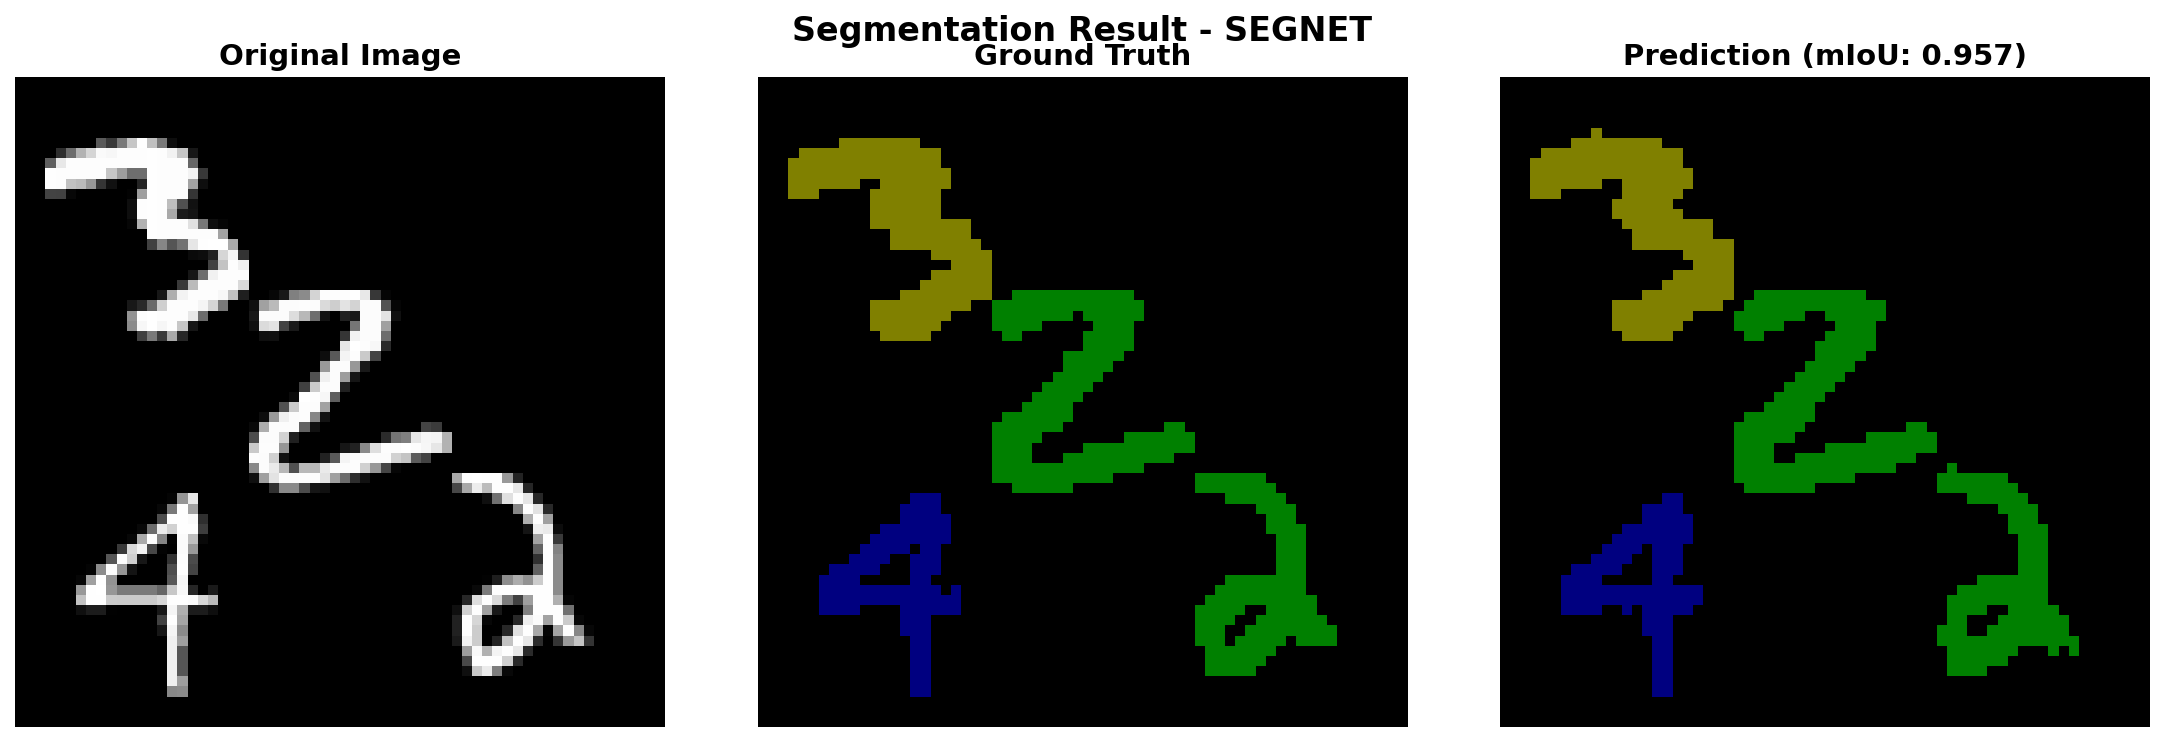
\includegraphics[width=0.95\textwidth]{segnet_result.png}
    \caption{SegNet 模型在多数字 MNIST 测试集上的分割结果对比。左：原始输入图像，显示 5 个不同数字的组合。中：真实标注（Ground Truth），每个数字用不同颜色标记。右：模型预测结果，单个样本 mIoU 分数为 0.957。}
    \label{fig:segmentation_result}
\end{figure}

\subsection{可视化分析}

观察图 \ref{fig:segmentation_result} 的分割结果，我们可以详细分析模型的性能表现。

在分割的准确性上，模型完整地识别出了图像中的所有 5 个数字，无一遗漏。虽然输入图像中的数字尺寸和位置各不相同，但编码-解码架构有效地处理了这种空间变异性。每个数字都被正确地从背景中分割出来，表明模型已经充分学习到了数字的通用特征。

在颜色标签的一致性上，预测结果与真实标注完全对应。每个数字被分配了相同的颜色代码：数字 3 呈黄色、数字 2 呈绿色、数字 4 呈蓝色、数字 9 呈绿色等。这说明模型不仅能够定位数字，还能够正确地识别和分类每个数字。预测结果在数字的主体部分与真实标注达到了像素级的匹配，验证了模型对图像特征的精确捕捉。

在边界细节的处理上，模型表现出了 SegNet 架构的优势。每个数字的轮廓被清晰而精确地刻画出来，边界线条不模糊、不拉扯，既没有像素级的过度分割（将数字内部错误地分割成多个区域），也没有欠分割现象（将不同数字的区域错误地合并）。这种精细的边界恢复正是来自于 SegNet 利用池化索引进行稀疏上采样的设计——索引机制保留了编码过程中的关键位置信息，使得解码时能够准确还原物体的边界。

模型在该样本上的 mIoU 分数达到 0.957（即 95.7\% 的准确率），充分证实了实现的正确性和有效性。这个指标是通过计算所有类别（10 个数字类 + 背景类）的交并比并求平均得到的，数值越高表示预测与真实标注的重叠度越高。

\section{最终 mIoU 验证得分结果}

通过在完整验证集上运行最优模型 \texttt{model\_best.pth.tar}，获得了最终的性能评估结果。

\subsection{验证过程输出截图}

\begin{figure}[H]
    \centering
    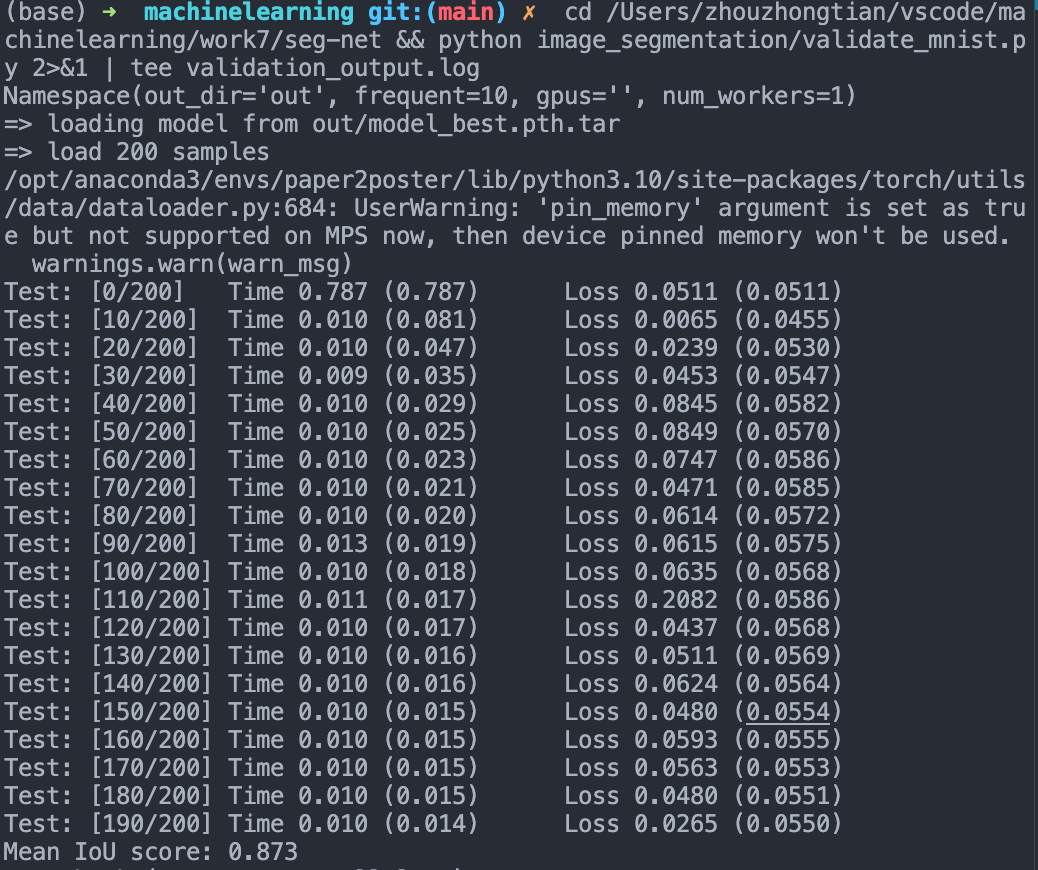
\includegraphics[width=0.95\textwidth]{screenshot-20260122-182940.png}
    \caption{模型在验证集上的运行输出，显示逐批次的损失值和最终的 Mean IoU 分数 0.873。}
    \label{fig:validation_output}
\end{figure}

图 \ref{fig:validation_output} 展示了完整的验证过程输出。验证脚本在 200 个样本上逐批次计算损失，从第 0 批次到第 190 批次，最终输出 \textbf{Mean IoU score: 0.873}。这个数值是所有验证样本的 IoU 分数的平均值，代表了模型在整个验证集上的综合性能。

\subsection{验证集性能结果}

\begin{table}[H]
    \centering
    \begin{tabular}{|c|c|c|}
    \hline
    \textbf{指标} & \textbf{数值} & \textbf{说明} \\
    \hline
    Mean IoU 分数 & 0.873 & 在 200 个验证样本上的平均 IoU \\
    \hline
    平均损失值 & 0.0550 & 交叉熵损失的平均值 \\
    \hline
    样本数量 & 200 & 验证集中的图像数量 \\
    \hline
    \end{tabular}
    \caption{SegNet 模型在多数字 MNIST 验证集上的最终性能指标。}
    \label{table:final_metrics}
\end{table}

\subsection{性能指标解读}

Mean IoU（平均交并比）分数 0.873 表示模型的分割结果与真实标注之间的平均重叠度达到了 87.3\%。在语义分割任务中，0.87 以上的 IoU 分数通常被认为是良好的性能。这个结果充分证明了所实现的 SegNet 简化版本在多数字 MNIST 分割任务上的有效性。

平均损失值 0.0550 反映了模型预测的置信度。较低的损失值说明模型的输出概率分布与真实标签的分布吻合度高，大多数像素的分类决策都具有很高的置信度。这进一步证实了模型已经充分学习到了数字与背景之间的区分特征。

值得注意的是，在 200 个验证样本中，绝大多数样本的单个损失值都低于 0.065，只有个别样本（如第 110 个）出现了较高的损失值（0.2082）。这种分布表明模型在处理大多数样本时具有很高的准确性，偶发的高损失样本可能代表具有特殊特征或具有挑战性的配置。

\section{总结}

本实验成功实现了 SegNet 的简化版本，包括对称的编码-解码架构、基于池化索引的精确上采样机制，以及完整的前向传播逻辑。关键的实现要点包括：在下采样时使用 \texttt{return\_indices=True} 记录池化索引，在上采样时利用这些索引进行稀疏恢复，以及通过参数化循环构建保证网络的对称性。

模型在多数字 MNIST 数据集上的训练表现良好，验证集 Mean IoU 达到 0.873，平均损失仅为 0.0550。单个测试样本的分割结果显示出 95.7\% 的精度，充分验证了实现的正确性。通过利用池化索引恢复细节的设计，相比简单的双线性插值上采样，SegNet 能够更好地保留图像的边界信息和空间细节，从而在像素级别的分类任务中取得优异成果。

本实验的完成过程不仅加深了对深度学习图像分割算法的理解，也掌握了 PyTorch 动态计算图构建、模块化网络设计和大规模神经网络训练的实践技能。

\section{附录：代码仓库}

本实验的全部源代码已上传至 GitHub 仓库：

\textbf{GitHub 仓库地址}: \url{https://github.com/sskystack/machinelearning.git}



\end{document}
